\documentclass{article}
\usepackage{epsfig,graphicx,epsf,subfigure, amssymb, amsmath, float}
\usepackage{hyperref}
\usepackage[letterpaper, total={6.5in, 9in}]{geometry}
\author{Oscar Wang, David Zhou, Andrew Gauthier, David Zhang}
\date{\today}
\title{ECE 458 Evolution 3 Write Up}
\begin{document}
\maketitle
\section{Design Choices}
\subsection{Ruby on Rails}
Once again, we have mixed feelings about Ruby on Rails for this evolution.  On one hand, Ruby on Rails was designed to create web applications like this, and sometimes it is clear to see why it is such a popular choice of technology.  It allows us to quickly modify our code and satisfy many of the requirements in a short amount of time.  Within hours, we were able to get many of the features implemented, and we probably would not have been able to push out functional code faster with any other language.  Ruby has many nice features, including support for functional-programming-like operations and clean and readable syntax.  However, it also has its flaws; although types in Ruby exist, they are not declared, which makes testing and debugging a bit of a pain.\par
While Ruby on Rails has proven useful in each evolution for writing code quickly, it has certainly hurt us toward the end of the evolutions.  The hardest features in each evolution have been extremely difficult to implement because our understanding of Ruby on Rails is not perfect, or even as good as we initially thought.  Part of the reason for this is that most of our knowledge of Ruby on Rails is self-taught, while we have been using languages like Java for Duke classes for years.  This makes it difficult for us to figure out how to solve problems that are not well documented on the web.  For example, setting up OAuth2, a requirement from Evolution 2, is still giving us problems because of problems with the Devise gem, which filters out access to parameters as a security measure.  Furthermore, debugging has also taken an extremely long time. Many of the bugs are caused by our incomplete understanding of Ruby on Rails, and we have not been able to use the debugging tools as effectively as we would like.  The lack of an IDE also makes coding and debugging our code a little more difficult, and sometimes we actually miss the Eclipse IDE.\par
One of the considerations we had was redoing our project using a new framework and a language we are a stronger understanding of.  However, we ultimately ruled against it because our application still has most of the functionality already implemented, and many of our problems are also related to our inexperience with HTML, CSS, and JavaScript, which we would have to deal with using another framework.  Furthermore, we would have to reimplement 3 evolutions worth of features at this point if we started over.  Although Ruby on Rails has its problems, it has also made some things easier for us, and our application is not such a train wreck that it is worth discarding the entire thing.
\subsection{PostgreSQL and Heroku}
We have had no further problems with PostgreSQL and Heroku, and it seems like we will continue to use them.  We still do not know what causes our server to time out on the virtual machines, and we have decided that a better use of our time is trying to implement all of the features and iron out all of the bugs.  Given the current state of our application, we need to focus on the bigger problems at hand, and not having to worry about the technologies we are using will help with that.
\section{Program Organization}
\begin{figure}[h]
\centering
\includegraphics[width=5in]{models}
\caption{Updated Interactions Between the Design Models}
\end{figure}
\subsection{Models}
Our models changed somewhat since the previous evolution to adjust to the changed requirements. A reservation now has a many to many relationship with resources, due to the new requirement of a reservation containing multiple resources. This also required some changes to how we check for conflicts between reservations, as we must now check the current bookings on all resources involved. We also added functionality in the permission model to handle the new resource specific permission for accepting restricted reservations. In doing so, we extended on the group permission model from before. There are now two kinds of groups: regular groups that the user sees and ``hidden'' groups that only contain one person and are hidden to the user.  Since many of the requirements involving permissions treat individuals and groups the same, we thought that this would be a fine way to give the same functionality to both without duplicating code.  With this design, there is just have one relationship with permissions--a many to many relationship with groups--and no additional user to permissions relationships.  In the last evolution, it may be worth trying to see if we can come up with something that removes the unintuitive aspect of the design, where a user and the permissions associated with that user live in separate models.  This already gave us problems during the debugging process, where deleting a user was not deleting its hidden group.  There may be smarter ways of tackling this problem that involve features of Ruby on Rails that we are not familiar with.  Other than this dilemma, our design satisfies all of the additional requirements for the models while trying to remain as open to extension as possible, so the models should be in good shape for the final evolution.

\subsection{Controllers}
We added functionality for the multiple resource per reservation requirement, which mainly involved the reservation controller, and also added in functionality for approving restricted reservations. This approve method also works to identify and delete the other oversubscribed reservations, if they exist.  Using Ruby on Rails's standard controller formatting allowed us to implement many basic features very quickly, since it only takes a few lines of code to implement standard operations such as create, update, delete, and edit.  Using the standard Ruby on Rails MVC design will continue to make implementing these simple operations very easy in the future, but we anticipate that we will continue to struggle with the harder features.  For example, we struggled for a long time to figure out how to implement listeners that could retain the old value of a variable after an update call.  While this would be simple to write in Java, it caused us a lot of difficulty to figure out how to do it in Ruby on Rails.  To avoid repeating this problem in the final evolution, it might be beneficial to spend more time learning about the proper way to perform these tasks in Ruby, instead of trying to hack together a solution from online documentation.  The approach we have been trying has been quite inefficient, and has been responsible for some of the bugs in our project.

\subsection{Views}

We have done a lot of work to make the front end more intuitive.  While the Twitter Bootstrap was used to create many of the visual elements in our user interface, the actual data from the backend was queued using embedded Ruby on Rails code in our view files.  This approach has made it extremely easy to add new information to the front end, since the variables are named exactly the same as in the controller.  It has also served as a crutch for our lack of experience with HTML, CSS, and JavaScript; by having Ruby on Rails render much of the HTML and JavaScript for us, we did not have to dedicate as much time to learning new languages for the front end of our application.  However, it might have been a good thing if we learned a little more about these three languages, especially given how important they are to web design.  Our lack of experience with JavaScript is one of the reasons we still have not yet managed to implement OAuth2 sign-in.\par

Furthermore, the view classes are extremely long because of all the Twitter Bootstrap HTML elements that we included in our front end.  Many of the portions of the code look very similar, especially all of the tables that we use to display our data.  Although some of the code is almost duplicated, we do not yet know how to use functions to allow us to repeatedly render the similar sections while keeping the elements that are different between them distinct.  For the final evolution, it may be worth looking into this, because it would save us time in the long run when we make modifications to similar front end elements.  For example, the table of resources on the ``Reservations'' and ``Resources'' pages are very similar, but have slightly different table entries.  If we could refactor this table into the HTML equivalent of a function, we would be able to make edits to both tables more easily.\par

Overall, we are happy with the progress to the front end during this evolution.  It is a lot more user friendly, since the tabs and links are much more intuitively organized.  In addition, the front end also combines elements from the back end and presents it in a way that is understandable to the user; for example, while users exists as both a user and a group in the back end, the front end combines this information into a single table so that the user of the application is not aware of this.  This process was relatively painless because of the use of embedded Ruby code in our front end, and we anticipate that this feature will continue to facilitate extending our front end.

\section{Evaluation and Future Plans}
At this point, our app still has some very big weaknesses.  While the code is simple and modular, there are still several bugs that need to be fixed.  Many of them are not a result of poor coding practices (Ruby on Rails does a lot to prevent that using its built in MVC organization) but just lack of experience with some of the methods available to us.  The biggest bugs that remain are
\begin{itemize}
\item{The date range selector from evolution 1, which we finally got around to trying to implement, is suffering from a glitch that makes it nonfunctional.}
\item{Overlapping resources are not always properly detected.  We believe that this has to do with the model not properly referring to the old or new value of a start time or end time when one of the values has changed, but we are not sure how to implement a listener that can handle this into our models.}
\item{The database may not always be properly updated when we destroy a object.  For example, tags would persist when all resources bearing that tag were destroyed and ``hidden'' users discussed earlier would remain when their corresponding user was destroyed.  We have found and fixed many of these bugs, and all of the ones we were aware of have been fixed, but there may be others out there that we have not caught yet.}
\end{itemize}
These bugs have slowed us down a lot, and prevented us from spending as much time as we would like on implementing actual features and requirements.  As of right now, there are many features from the first two requirements that we have not been able to dedicate enough time to.  In particular, the two features from the first two evolutions (time-range selection and OAuth2) that we have wanted to fix for the last few weeks still have not been completely implemented, although we have come significantly closer to figuring out how implement them both.  We also need to do a lot more work on our API.  In particular, we need to make sure that it supports all of the interactions introduced in evolution 3 and document it more thoroughly.

\section{Plan}
\begin{figure}[h]
\centering
\includegraphics[width=6in]{schedule}
\caption{Proposed Work Schedule}
\end{figure}
Our plan for approaching the final evolution is to come up with a detailed plan and stick to it this time.  For the last evolution, we did not anticipate how unproductive we would become during spring break and did not accomplish as much as we hoped to.  Our proposed work schedule is presented above.  One of our biggest realizations is that debugging is one of the slowest steps in our coding process, so we are aiming to get the basic functionality implemented as soon as possible.  Hopefully, this will allow us ample time to fix any bugs that may arise so that we can focus on the most difficult requirements.\par

Overall, both the greatest strength and greatest weakness of our design is its simplicity.  Using a framework as simple and elegant as Ruby on Rails makes it very easy for us to quickly modify our code and implement basic extensions.  What we have realized at this point is that the amount of time it will take to complete the rest of project does not scale linearly with the number of requirements completed, because something is always going to go wrong with the last few.  Since this is the last evolution of the semester, we hope to do well on this one, so we can have a final product we can be proud of.

\section{Contributions}
\begin{itemize}
\item{Oscar Wang: Extended Models and Controllers, Debugging}
\item{David Zhou: Extensions on the front end, Debugging, Write-Up}
\item{Andrew Gauthier: Extended Models, Figures}
\item{David Zhang: Extended Models, Presentation}
\end{itemize}
\section{Appendix}

\begin{figure}[h]
\centering
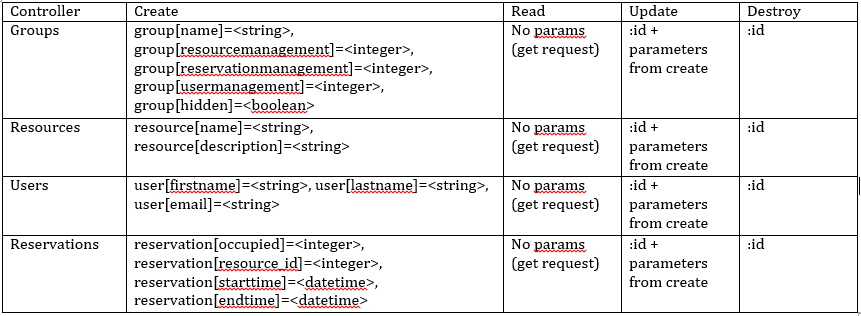
\includegraphics[width=6in]{table}
\caption{API}
\end{figure}

\end{document}

